\scanpage{28}
b) Context of finite families of quadratic modules : $=$ formula, with $=$ \unsure{proof|proof}

c) \diagram{\begin{tikzcd}[ampersand replacement=\&]
\deleted{I}J \arrow[r,"p"] \& I
\end{tikzcd}}
map \inserted{(surjection \unsure{if one wishes})} of \deleted{\unsure{C|f}}finite sets,
\[
 I^{-}=\{i\in I\mid\operatorname{Card}p^{-1}(i)\ \text{odd}\}.
\]
\deleted{\unsure{I say that}} [for example $J$ set with equivalence relation \inserted{$\mathcal R$}, and $I=J/\mathcal R$]. \deleted{\unsure{O}}Then
\[
 \omega_J\simeq\omega_{I^{-}}\wedge\bigwedge_{i\in I}\omega_{J_{\unsure{2|i}}}
\]
% slanted broken traces at the right; one estimated unreadable unit
\margin{\illegible{1}}

\uline{\unsure{Compatibilities|Compatibility}} between the \unsure{canonical|cas.} isomorphisms a) b) c)

\figure{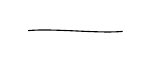
\begin{tikzpicture}
\draw (0,0) .. controls (.32,.03) and (.92,-.04) .. (1.2,-.01);
\end{tikzpicture}}

\uline{Case of extensions}
\[
 \{0\}=\deleted{\unsure{0}}E_0\subset E_1\subset E_2\ \mathinner{\cdotp\cdotp}\ \subset E_d=E
\]
\deleted{\unsure{One}} Define a canonical isomorphism
\[
 \omega_E\simeq\bigwedge_{1\leq i\leq d}\omega_{E_i\unsure{/|{}}E_{i-1}}
\]
\figure{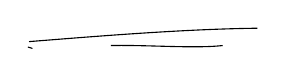
\begin{tikzpicture}
\draw (0,0) .. controls (.76,.06) and (1.95,.16) .. (2.90,.17);
\draw (1.04,-.05) .. controls (1.50,-.04) and (2.10,-.09) .. (2.46,-.05);
\draw[line cap=round] (-.01,-.07) -- (.04,-.085);
\end{tikzpicture}}
% archive sheet number: 27
